\chapter{Background}
\label{chap:background}

In this chapter, we provide background knowledge that is commonly used across this dissertation.
Preliminaries specific to each chapter will be introduced later when they are needed.
Symbols used in this dissertation are summarized in~\cref{tbl:symbols}.

\begin{table}[t]
    \centering
    \caption{A summary of symbols used in the dissertation}
    \label{tbl:symbols}
    \begin{tabular}{c|c}
        Symbol                      & Description                                                 \\
        \hline
        $\booldom$                  & The Boolean domain $\{\bot,\top\}$                          \\
        $x$                         & A Boolean variable                                          \\
        $l$                         & A literal (a variable or its negation)                      \\
        $\vl{l}$                    & The variable of $l$                                         \\
        $\as$                       & An assignment (a mapping from a variable set to $\booldom$) \\
        $\as(x)$                    & The assigned value of $x$                                   \\
        $\av{V}$                    & The set of all assignments over variable set $V$            \\
        $\pf$                       & A quantifier-free formula                                   \\
        $\vf{\pf}$                  & The set of variables appearing in $\pf$                     \\
        $\as\models\pf$             & $\as$ satisfies $\pf$                                       \\
        $\pcf{\pf}{x},\ncf{\pf}{x}$ & Positive and negative cofactors of $\pf$ w.r.t. $x$         \\
        $C$                         & A clause (a disjunction of literals)                        \\
        $\qf$                       & A quantified formula                                        \\
    \end{tabular}
\end{table}

\section{Propositional logic}
\label{sect:background-propositional-logic}

We denote Boolean constants \false and \true by symbols $\bot$ and $\top$, respectively.
In arithmetic expressions, $\bot$ is interpreted as integer $0$ and $\top$ as integer $1$.
A variable $x$ that takes values from the Boolean domain $\booldom=\{\bot,\top\}$ is called a Boolean variable.
A \textit{literal} is a variable itself (a \textit{positive} literal) or the negation of a variable (a \textit{negative} literal).
For a literal $l$, let $\vl{l}$ denote the variable of $l$.
Boolean connectives $\lnot, \lor, \land, \limply, \equiv$ are used under their conventional semantics.
Over a finite set $V$ of Boolean variables,
we define a \textit{well-formed formula} $\pf$ with the following Backus-Naur-form (BNF) grammar:
\begin{align}
    \pf ::= x\in V | \lnot\pf | (\pf\lor\pf) | (\pf\land\pf) | (\pf\limply\pf) | (\pf\equiv\pf).
\end{align}
Given a well-formed formula $\pf$, let $\vf{\pf}$ denote the set of Boolean variables appearing in $\pf$.
In the following, a variable is Boolean if not otherwise specified.
We shall consider well-formed formulas only and refer to them as \textit{Boolean formulas}.

\subsection{Conjunctive and disjunctive normal form}
Among various representations of a Boolean formula,
we are particularly interested in normal-form representations because their simplicity allows efficient analyses.

A Boolean formula is in \textit{conjunctive normal form} (CNF) if it is a conjunction of \textit{clauses},
where a clause is a disjunction of literals.
A Boolean formula is in \textit{disjunctive normal form} (DNF) if it is a disjunction of \textit{cubes},
where a cube is a conjunction of literals.
A variable $x$ is said to be \textit{pure} in a formula if its appearances in the formula are all positive literals or negative literals.
We alternatively treat a clause or a cube as a set of literals,
and a CNF (resp. DNF) formula as a set of clauses (resp. cubes).
In the rest of the dissertation, a Boolean formula is assumed to be given in CNF if not otherwise specified.

\subsection{Boolean satisfiability}
An \textit{assignment} $\as$ over a variable set $V$ is a mapping from $V$ to $\booldom$.
We denote the set of all assignments over $V$ by $\av{V}$.
Given a Boolean formula $\pf$,
an assignment $\as$ over $\vf{\pf}$ is called a \textit{complete} assignment for $\pf$.
If $\as$ is over a proper subset of $\vf{\pf}$, it is called a \textit{partial} assignment.
The resultant formula of $\pf$ induced by an assignment $\as$ over a variable set $V$,
denoted as $\pcf{\pf}{\as}$,
is obtained via substituting the occurrences of every $x\in V$ in $\pf$ with its assigned value $\as(x)$.
Such substitution is called \textit{cofactoring} $\pf$ with $\as$.
If $V=\{x\}$, we write $\pcf{\pf}{x}$ (resp. $\ncf{\pf}{x}$) to denote the resultant formula of $\pf$ under an assignment that maps $x$ to $\top$ (resp. $\bot$),
and call this formula the \textit{positive} (resp. \textit{negative}) \textit{cofactor} of $\pf$ with respect to variable $x$.

A complete assignment $\as$ \textit{satisfies} $\pf$, denoted as $\as\models\pf$, if $\pcf{\pf}{\as}=\top$.
Such complete assignment $\as$ is called a \textit{satisfying complete assignment} for $\pf$.
On the other hand, if $\pcf{\pf}{\as}=\bot$, $\as$ is called an \textit{unsatisfying complete assignment}.
Similarly, a partial assignment $\as^+$ over $X\subset\vf{\pf}$ is called a \textit{satisfying} (resp. an \textit{unsatisfying}) \textit{partial assignment} for $\pf$
if for some (resp. every) assignment $\mu$ over $\vf{\pf}\setminus X$,
$\pf$ valuates to $\top$ (resp. $\bot$) under the complete assignment that combines $\as$ and $\mu$.
We alternatively represent an assignment $\as$ for $\pf$ as a cube.
A cube is called a \textit{minterm} of formula $\pf$ when it corresponds to a complete assignment over $\vf{\pf}$.
Given two Boolean formulas $\pf_1$ and $\pf_2$ over a same set $V$ of variables,
we write $\pf_1\limply\pf_2$ if the following condition holds:
$\forall\as\in\av{V}.\as\models\pf_1\limply\as\models\pf_2$.

A Boolean formula $\pf$ is \textit{satisfiable} if it has a satisfying complete assignment.
Otherwise, $\pf$ is \textit{unsatisfiable}.
A Boolean formula $\pf$ is a \textit{tautology} if the following condition holds:
$\forall\as\in\av{\vf{\pf}}.\as\models\pf$.
The Boolean satisfiability problem asks to decide whether a Boolean formula is satisfiable or not.
It is a well-known NP-complete~\cite{Cook1971} problem.
We write $\sat{\pf}$ (resp. $\unsat{\pf}$) to indicate $\pf$ is satisfiable (resp. unsatisfiable).
A satisfying complete assignment of $\pf$ is also called a \textit{model} of $\pf$, which is denoted by $\model{\pf}$.

A set $\base\subseteq\vf{\pf}$ is a \textit{base set} for $\pf$ if
for any (partial) assignment $\as^+$ over $\base$,
there exists at most one assignment $\mu$ over $\vf{\pf}\setminus\base$
such that $\pf$ is satisfied by the combined assignment of $\as^+$ and $\mu$ over $\vf{\pf}$.
Observe that, given any Boolean formula $\pf$,
a base set must exist ($\vf{\pf}$ is a trivial base set of $\pf$) but may not be unique.
Let $\as^+$ be an assignment over a base set $\base\subseteq\vf{\pf}$.
If there exists an assignment $\mu$ over $\vf{\pf}\setminus\base$
such that the combined assignment $\nu$ satisfies $\pf$,
then we say that $\pf$ is satisfiable under $\as^+$ and write $\as^+\models\pf$ to mean $\nu\models\pf$.
If there does not exist such an assignment $\mu$ over $\vf{\pf}\setminus\base$,
then $\pf$ is unsatisfiable under $\as^+$, denoted by $\as^+\not\models\pf$.

An $n$-variable \textit{Boolean function} is a mapping from $\booldom^n$ to $\booldom$.
Note that a Boolean formula $\pf$ induces a Boolean function with a domain $\av{\vf{\pf}}$.
We shall not distinguish between a Boolean formula and its induced Boolean function.
\section{Model counting}
\label{sect:related-work-model-counting}

Model-counting~\cite{SATHandbook-ModelCounting} algorithms can be classified into two categories:
exact counting and approximate counting.
The former adopts DPLL-based search with additional techniques,
such as component analysis and caching, to improve the counting efficiency\cite{Sang2004,Sang2005ModelCounting}.
The latter takes a different strategy,
aiming at providing lower and/or upper bounds with guarantee on confidence level.
Ideas from statistics~\cite{Chakraborty2016} have been adopted to increase the capacity limit of model counting.

There are many variants of model counting.
For example,
weighted model counting asks to aggregate the weight of every satisfying assignment.
It has been widely adopted in probabilistic inference~\cite{Sang2005BayesianInference,Chavira2008}.
\textit{Projected model counting}~\cite{Aziz2015} computes the numbers of satisfying assignments
projected on a subset of original variables.
\textit{Maximum model counting}~\cite{Fremont2017} finds an assignment to a subset of variables in a formula
such that the number of satisfying assignments of the residual formula cofactored with the assignment is maximized.

The above variants of model counting can be expressed via SSAT,
because the randomized quantifiers of SSAT essentially aggregate the results from different branches with weights.
\Cref{tbl:related-work-model-counting} shows the variants of model-counting problems and their respective SSAT encodings.
Note that projected weighted model counting and maximum weighted model counting are equivalent to
random-exist quantified SSAT and exist-random quantified SSAT, respectively.

\begin{table}[t]
    \centering
    \caption{Model-counting variants and their corresponding SSAT formulas}
    \label{tbl:related-work-model-counting}
    \begin{tabular}{c|c}
        Model-counting variant & SSAT encoding                                                                                              \\
        \hline
        Unweighted             & $\random{0.5}x_1,\ldots,\random{0.5}x_n.\pf(x_1,\ldots,x_n)$                                               \\
        Weighted               & $\random{p_1}x_1,\ldots,\random{p_n}x_n.\pf(x_1,\ldots,x_n)$                                               \\
        Projected              & $\random{0.5}x_1,\ldots,\random{0.5}x_n,\exists y_1,\ldots,\exists y_m.\pf(x_1,\ldots,x_n,y_1,\ldots,y_m)$ \\
        Maximum                & $\exists x_1,\ldots,\exists x_n,\random{0.5}y_1,\ldots,\random{0.5}y_m.\pf(x_1,\ldots,x_n,y_1,\ldots,y_m)$ \\
        Projected weighted     & $\random{p_1}x_1,\ldots,\random{p_n}x_n,\exists y_1,\ldots,\exists y_m.\pf(x_1,\ldots,x_n,y_1,\ldots,y_m)$ \\
        Maximum weighted       & $\exists x_1,\ldots,\exists x_n,\random{p_1}y_1,\ldots,\random{p_m}y_m.\pf(x_1,\ldots,x_n,y_1,\ldots,y_m)$ \\
    \end{tabular}
\end{table}

The latest developments of model counting can be found in the report~\cite{MC-COMP2020} of the 2020 Model Counting Competition.
\begin{frame}
    \frametitle{Background}
    \begin{block}{Stochastic Boolean Satisfiability (SSAT)}
        $\Qf=Q_1 x_1,\ldots,Q_n x_n.\pf$
        \pause
        \begin{itemize}
            \item $Q_1 x_1,\ldots,Q_n x_n$: quantification structure, $Q_i \in \{\random{p},\exists\}$ (\emph{prefix})
                  \pause
            \item $\pf$: quantifier-free formula over $\{x_1,\ldots,x_n\}$ (\emph{matrix})
        \end{itemize}
    \end{block}
    \pause
    \begin{block}{Computational Rules for Satisfying Probability}
        Let $x$ be the outermost variable in the prefix:
        \pause
        \begin{enumerate}
            \item[a)] $\spb{\top}=1$,
                  \pause
            \item[b)] $\spb{\bot}=0$,
                  \pause
            \item[c)] $\spb{\Qf}=\max\{\spb{\ncf{\Qf}{x}},\spb{\pcf{\Qf}{x}}\}$, if $x$ is quantified by $\exists$,
                  \pause
            \item[d)] $\spb{\Qf}=(1-p)\spb{\ncf{\Qf}{x}}+p\spb{\pcf{\Qf}{x}}$, if $x$ is quantified by $\random{p}$.
        \end{enumerate}
    \end{block}
\end{frame}

\begin{frame}
    \frametitle{Background}
    \begin{block}{Example: Computation of Satisfying Probability}
        \abovedisplayskip=0pt
        \begin{align*}
             & \Qf=\random{0.5} x_1, \exists y_1, \random{0.5} x_2, \exists y_2. \pf \\
             & \pf=(x_1 \lor \lnot y_1)
            (\lnot x_1 \lor y_1)
            (\lnot x_1 \lor \lnot x_2 \lor y_2)
            (x_1 \lor \lnot y_2)
            (x_2 \lor \lnot y_2)
        \end{align*}
    \end{block}\pause
    \begin{figure}
        \centering
        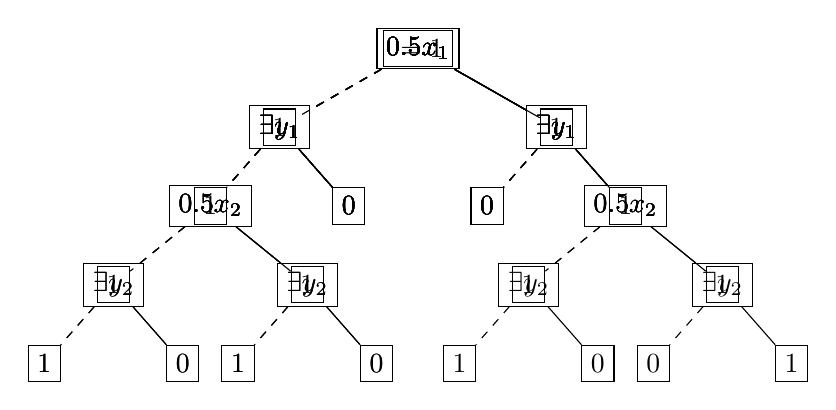
\begin{tikzpicture}[
                baseline,
                level distance=10mm,
                level 1/.style={sibling distance=10em},
                level 2/.style={sibling distance=5em},
                level 3/.style={sibling distance=7em},
                level 4/.style={sibling distance=5em},
                every node/.style={solid,draw},
                positive/.style={edge from parent/.style={solid,draw}},
                negative/.style={edge from parent/.style={dashed,draw}}]

            \action<2>{\node{$\random{0.5} x_1$};}
            \action<3>{\node{$\random{0.5} x_1$}
                child[negative]{node{$\exists y_1$}}
                child[positive]{node{$\exists y_1$}};}
            \action<4>{\node{$\random{0.5} x_1$}
                child[negative]{node{$\exists y_1$}
                        child[negative]{node{$\random{0.5} x_2$}}
                        child[positive]{node{$0$}}}
                child[positive]{node{$\exists y_1$}};}
            \action<5>{\node{$\random{0.5} x_1$}
                child[negative]{node{$\exists y_1$}
                        child[negative]{node{$\random{0.5} x_2$}}
                        child[positive]{node{$0$}}}
                child[positive]{node{$\exists y_1$}
                        child[negative]{node{$0$}}
                        child[positive]{node{$\random{0.5} x_2$}}};}
            \action<6>{\node{$\random{0.5} x_1$}
                child[negative]{node{$\exists y_1$}
                        child[negative]{node{$\random{0.5} x_2$}
                                child[negative]{node{$\exists y_2$}
                                        child[negative]{node{$1$}}
                                        child[positive]{node{$0$}}}
                                child[positive]{node{$\exists y_2$}
                                        child[negative]{node{$1$}}
                                        child[positive]{node{$0$}}}}
                        child[positive]{node{$0$}}}
                child[positive]{node{$\exists y_1$}
                        child[negative]{node{$0$}}
                        child[positive]{node{$\random{0.5} x_2$}}};}
            \action<7>{\node{$\random{0.5} x_1$}
                child[negative]{node{$\exists y_1$}
                        child[negative]{node{$\random{0.5} x_2$}
                                child[negative]{node{$\exists y_2$}
                                        child[negative]{node{$1$}}
                                        child[positive]{node{$0$}}}
                                child[positive]{node{$\exists y_2$}
                                        child[negative]{node{$1$}}
                                        child[positive]{node{$0$}}}}
                        child[positive]{node{$0$}}}
                child[positive]{node{$\exists y_1$}
                        child[negative]{node{$0$}}
                        child[positive]{node{$\random{0.5} x_2$}
                                child[negative]{node{$\exists y_2$}
                                        child[negative]{node{$1$}}
                                        child[positive]{node{$0$}}}
                                child[positive]{node{$\exists y_2$}
                                        child[negative]{node{$0$}}
                                        child[positive]{node{$1$}}}}};}
            \action<8>{\node{$\random{0.5} x_1$}
                child[negative]{node{$\exists y_1$}
                        child[negative]{node{$\random{0.5} x_2$}
                                child[negative]{node{$1$}}
                                child[positive]{node{$1$}}}
                        child[positive]{node{$0$}}}
                child[positive]{node{$\exists y_1$}
                        child[negative]{node{$0$}}
                        child[positive]{node{$\random{0.5} x_2$}
                                child[negative]{node{$1$}}
                                child[positive]{node{$1$}}}};}
            \action<9>{\node{$\random{0.5} x_1$}
                child[negative]{node{$\exists y_1$}
                        child[negative]{node{$1$}}
                        child[positive]{node{$0$}}}
                child[positive]{node{$\exists y_1$}
                        child[negative]{node{$0$}}
                        child[positive]{node{$1$}}};}
            \action<10>{\node{$\random{0.5} x_1$}
                child[negative]{node{$1$}}
                child[positive]{node{$1$}};}
            \action<11>{\node{$\spb{\Qf}=1$};}
        \end{tikzpicture}
    \end{figure}
\end{frame}

\begin{frame}
    \frametitle{Express Model-Counting Variants with SSAT}
    \begin{table}[t]
        \centering
        \begin{tabular}{c|c}
            Variant            & SSAT encoding                                                               \\
            \hline
            Unweighted         & $\random{0.5}x_1,\ldots,\random{0.5}x_n.\pf$                                \\
            Weighted           & $\random{p_1}x_1,\ldots,\random{p_n}x_n.\pf$                                \\
            Projected          & $\random{0.5}x_1,\ldots,\random{0.5}x_n,\exists y_1,\ldots,\exists y_m.\pf$ \\
            Maximum            & $\exists x_1,\ldots,\exists x_n,\random{0.5}y_1,\ldots,\random{0.5}y_m.\pf$ \\
            Projected weighted & $\random{p_1}x_1,\ldots,\random{p_n}x_n,\exists y_1,\ldots,\exists y_m.\pf$ \\
            Maximum weighted   & $\exists x_1,\ldots,\exists x_n,\random{p_1}y_1,\ldots,\random{p_m}y_m.\pf$ \\
        \end{tabular}
    \end{table}
\end{frame}

\begin{frame}
    \frametitle{Background}
    \begin{block}{Game-Theoretical Interpretation of SSAT}
        $\Qf=Q_1 x_1,\ldots,Q_n x_n.\pf$, $Q_i \in \{\random{p},\exists\}$
        \pause
        \begin{itemize}
            \item $\random{p}$: nondeterministic factors
                  \pause
            \item $\exists$: an agent who plays under uncertainty
                  \pause
            \item $\pf$: game matrix
                  \pause
            \item $\spb{\Qf}$: the maximum winning probability of the agent
                  \pause
            \item \alert{Skolem functions}: a winning/optimization strategy of the agent
        \end{itemize}
    \end{block}\pause
    \begin{block}{Example: Skolem Functions}
        \abovedisplayskip=0pt
        \belowdisplayskip=0pt
        \begin{align*}
             & \Qf=\random{0.5} x_1, \exists y_1, \random{0.5} x_2, \exists y_2. \pf \\
             & \pf=(x_1 \lor \lnot y_1)
            (\lnot x_1 \lor y_1)
            (\lnot x_1 \lor \lnot x_2 \lor y_2)
            (x_1 \lor \lnot y_2)
            (x_2 \lor \lnot y_2)
        \end{align*}
        \pause
        \begin{itemize}
            \item Variable $y_1$: $f_1(x_1)=x_1$; variable $y_2$: $f_2(x_1,x_2)=x_1 \land x_2$
        \end{itemize}
    \end{block}
\end{frame}
\section{Quantified Boolean formula}
\label{sect:qbf}

\subsection{Clause selection}
\textit{Clause selection}~\cite{Janota2015,Rabe2015} is a recently proposed technique for QBF solving.
Given a CNF formula $\phi(X,Y)$ over a set of variables $X \cup Y$ with $X \cap Y = \emptyset$, we divide each clause $C \in \phi$ into two sub-clauses $C^X$ and $C^Y$, where $C^X$ (resp. $C^Y$) consists of the literals whose variables are in $X$ (resp. $Y$). For example, for $C=(x_1 \vee x_2 \vee y_1 \vee y_2)$, we have $C^X=(x_1 \vee x_2)$ and $C^Y=(y_1 \vee y_2)$. Clearly, $C=C^X \vee C^Y$.

A clause $C$ is said to be \emph{selected} by an assignment $\tau$ over $X$ if every literal in $C^X$ is assigned to $\bot$ by $\tau$; $C$ is said to be \emph{deselected} by $\tau$ if some literal in $C^X$ is assigned to $\top$ by $\tau$; $C$ is said to be \emph{undecided} if it is neither selected nor deselected.
We also use $\phi|_{\tau}$ to denote the set of clauses selected by the assignment $\tau$. A \emph{selection variable} $s_C$ is introduced for each clause $C$ and defined by $s_C \equiv \neg C^X$.
Hence, $s_C$ is an indicator of the selection of clause $C$.
That is, $s_C=\top$ (resp. $s_C=\bot$) indicates $C$ is selected (resp. deselected).
Let $S$ be the set of selection variables for clauses in $\phi(X,Y)$.
The formula $\psi(X,S)=\bigwedge_{C \in \phi}(s_C \equiv \neg C^X)$ is called the \emph{selection relation} of $\phi(X,Y)$.

\begin{example}\label{ex:select}
    Consider a CNF formula $\phi(X,Y)$ over two sets of variables $X=\{e_1,e_2,e_3\}$ and $Y=\{r_1,r_2,r_3\}$. $\phi(X,Y)$ consists of four clauses:
    \begin{itemize}
        \item[] $C_1: (e_1 \vee r_1 \vee r_2)$
        \item[] $C_2: (e_1 \vee e_2 \vee r_1 \vee r_2 \vee \neg r_3)$
        \item[] $C_3: (\neg e_2 \vee \neg e_3 \vee r_2 \vee \neg r_3)$
        \item[] $C_4: (\neg e_1 \vee e_3 \vee r_3)$
    \end{itemize}
    A selection variable $s_i$ is introduced for each clause, and $S=\{s_1,s_2,s_3,s_4\}$. The selection relation $\psi(X,S)$ of $\phi(X,Y)$ equals
    \begin{eqnarray*}
        \psi(X,S) = (s_1 \equiv \neg e_1)\wedge(s_2 \equiv \neg e_1 \wedge \neg e_2) \wedge (s_3 \equiv e_2 \wedge e_3) \\ \wedge(s_4 \equiv e_1 \wedge \neg e_3).
    \end{eqnarray*}
    Consider the complete assignment $\tau_1=\neg e_1 \neg e_2 \neg e_3$ over $X$. It selects $C_1$ and $C_2$, and deselects $C_3$ and $C_4$, as can be seen from the selection relation cofactored by $\tau_1$, which results in $\psi(X,S)|_{\tau_1}=s_1s_2\neg s_3 \neg s_4$.
    Consider the partial assignment $\tau_2=\neg e_1 e_3$ over $X$.
    It selects $C_1$, deselects $C_4$, and leaves $C_2$ and $C_3$ undecided.
    Notice that the two complete assignments $\neg e_1 \neg e_2 e_3$ and $\neg e_1 e_2 e_3$ consistent with $\tau_2$ select $\{C_1, C_2\}$ and $\{C_1, C_3\}$, respectively.
    The clause $C_1$ selected by the partial assignment $\tau_2$ lies in the intersection of the sets of clauses selected by the two complete assignments consistent with $\tau_2$.
\end{example}
\section{Dependency quantified Boolean formula}
\label{sect:dqbf}

In contrast to the \textit{linearly ordered} prefix used in QBF, i.e., an existentially quantified variable will depend on all of its preceding universally quantified variables,
the quantification structure in DQBF is extended with Henkin quantifiers,
where the dependency of an existentially quantified variable on the universally quantified variables can be explicitly specified.

A DQBF $\Phi$ over a set $V=\{x_1,\ldots,x_n,y_1,\ldots,y_m\}$ of variables is of the form:
\begin{align}
    \forall x_1, \ldots, \forall x_n, \exists y_1(D_{y_1}), \ldots, \exists y_m(D_{y_m}). \phi,
\end{align}
where each $D_{y_j}\subseteq \{x_1,\ldots,x_n\}$ denotes the set of variables that variable $y_j$ can depend on,
and Boolean formula $\phi$ over $V$ is quantifier-free.
We denote the set $\{x_1,\ldots,x_n\}$ (resp. $\{y_1,\ldots,y_m\}$) of universally (resp. existentially) quantified variables of $\Phi$ by $V_{\Phi}^\forall$ (resp. $V_{\Phi}^\exists$).

Given a DQBF $\Phi$, it is satisfied if for each variable $y_j$, there exists a function $f_j:\mathcal{A}(D_{y_j})\rightarrow \mathbb{B}$, such that after substituting variables in $V_{\Phi}^\exists$ with their corresponding functions respectively, matrix $\phi$ yields a tautology over $V_{\Phi}^\forall$.
The set of functions $\mathcal{F}=\{f_1,\ldots,f_m\}$ is called a set of \textit{Skolem} functions for $\Phi$.
In other words, $\Phi$ is satisfied by $\mathcal{F}$ if
\begin{align}\label{eq:dqbf-min}
    \min_{\beta \in \mathcal{A}(V_{\Phi}^{\forall})}\mathds{1}_{\phi|_{\mathcal{F}}}(\beta)=1,
\end{align}
where $\mathds{1}_{\phi|_{\mathcal{F}}}(\cdot)$ is an indicator function to indicate whether an assignment over $V_{\Phi}^{\forall}$ belongs to the set of satisfying assignments of matrix $\phi$,
when variables in $V_{\Phi}^{\exists}$ are substituted by their Skolem functions in $\mathcal{F}$.
That is, $\phi|_{\mathcal{F}} = \{\beta\ |\ \phi(\beta(x_1), \ldots, \beta(x_n)$, $f_1|_{\beta}$, $\ldots, f_m|_{\beta})\equiv \top\}$,
where $f_j|_{\beta}$ is the logical value derived by substituting every $x_i\in D_{y_j}$ with $\beta(x_i)$ in function $f_j$.
The satisfiability problem of DQBF was shown to be NEXPTIME-complete~\cite{Peterson2001}.
\section{Boolean-logic circuit}
\label{sect:circuit}

A Boolean-logic circuit, defined below, will be extended to model a probabilistic design in~\cref{chap:prob-eval}.

\begin{definition}[Boolean Network]\label{def:Boolean network}
    A \emph{(combinational) Boolean network} is a directed acyclic
    graph $G=(V,E)$, with vertices $V$ and edges $E \subseteq V \times
        V$. Two non-empty disjoint subsets $V_I$ and $V_O$ of $V$ are
    identified; a vertex $v \in V_I$ (resp. $V_O$) is referred to as a
    \emph{primary input} (PI) (resp. \emph{primary output} (PO)). Each
    vertex $v \in V$ is associated with a Boolean variable $b_v$; each
    vertex $v \in V \backslash V_I$ is associated with a Boolean
    function $f_v$ letting $b_v \leftrightarrow f_v$. An edge $(u,v)
        \in E$ indicates $f_v$ refers to $b_u$ as an input variable; $u$
    is called a \emph{fanin} of $v$, and $v$ a \emph{fanout} of $u$.
\end{definition}
To ease readability, in the sequel we shall not distinguish a
vertex $v$ and its corresponding Boolean variable $b_v$, and
simply denote $b_v$ with $v$.

For satisfiability (SAT) testing, a Boolean network (circuit) can
be converted in linear time to a \emph{conjunctive normal form}
(CNF) formula through Tseitin transformation~\cite{Tseitin1983},
which will be used in our development of stochastic SAT and model
counting methods.

\subsection{And-inverter graph}
\begin{frame}
      \frametitle{Modeling Decentralized POMDP}
      \begin{itemize}
            \item Multiple agents with uncertainty and partial information~\cite{Oliehoek2016}
                  \pause
            \item NEXPTIME-completeness~\cite{Bernstein2002}
                  \pause
            \item $\mathcal{M} = (I,S,\{A_i\},$ $T, \rho, \{O_i\}, \Omega, \Delta_0, h)$
                  \pause
                  \begin{itemize}
                        \item $T: S \times (A_1 \times \cdots \times A_n) \times S \mapsto [0,1]$
                              \pause
                        \item $\rho: S \times (A_1 \times \cdots \times A_n) \mapsto \mathbb{R}$
                              \pause
                        \item $\Omega: S \times (A_1 \times \cdots \times A_n) \times (O_1 \times \cdots \times O_n) \mapsto [0,1]$
                              \pause
                  \end{itemize}
            \item Optimal \emph{joint policy} to maximize the expected total reward
                  \pause
            \item A polynomial-time reduction from Dec-POMDP to DSSAT
                  \pause
                  \begin{itemize}
                        \item Extending the reduction from POMDP to SSAT~\cite{Salmon2020}
                  \end{itemize}
      \end{itemize}
\end{frame}

\begin{frame}
      \frametitle{Modeling Decentralized POMDP}
      \begin{center}
            \begin{tcolorbox}[colback=white]
    {\scriptsize
        \begin{align*}
             & \bigwedge_{0\leq t\leq h-2}[x_p^t \equiv \bot\rightarrow\bigwedge_{i\in I}x_o^{i,t} \equiv 0\wedge x_s^{t+1} \equiv 0\wedge x_p^{t+1} \equiv \bot]                                                                                                                                                       \\
             & x_p^{h-1}\equiv\bot                                                                                                                                                                                                                                                                                      \\
             & \bigwedge_{s\in S}\bigwedge_{\vec{a}\in\vec{A}}[x_p^0 \equiv\bot\wedge x_s^0 \equiv s \wedge\bigwedge_{i\in I}x_a^{i,0}\equiv a_i \rightarrow x_r^0 \equiv N_r(s,\vec{a})]                                                                                                                               \\
             & \bigwedge_{1\leq t\leq h-1}\bigwedge_{s\in S}\bigwedge_{\vec{a}\in\vec{A}}[x_p^{t-1}\equiv\top\wedge x_p^t \equiv\bot\wedge x_s^t \equiv s \wedge\bigwedge_{i\in I}x_a^{i,t}\equiv a_i\rightarrow
            x_r^t \equiv N_r(s,\vec{a})]                                                                                                                                                                                                                                                                                \\
             & \bigwedge_{0\leq t\leq h-2}\bigwedge_{s\in S}\bigwedge_{\vec{a}\in\vec{A}}\bigwedge_{s'\in S}[x_p^t \equiv \top\wedge x_s^t \equiv s \wedge\bigwedge_{i\in I}x_a^{i,t}\equiv a_i\wedge x_s^{t+1}\equiv s'\rightarrow x_{T_{s,\vec{a}}}^t \equiv s']                                                      \\
             & \bigwedge_{0\leq t\leq h-2}\bigwedge_{s'\in S}\bigwedge_{\vec{a}\in\vec{A}}\bigwedge_{\vec{o}\in\vec{O}}[x_p^t \equiv\top\wedge x_s^{t+1} \equiv s'\wedge\bigwedge_{i\in I}x_a^{i,t}\equiv a_i\wedge\bigwedge_{i\in I}x_o^{i,t}\equiv o_i\rightarrow x_{\Omega_{s',\vec{a}}}^t \equiv N_\Omega(\vec{o})]
        \end{align*}
    }
\end{tcolorbox}
      \end{center}
\end{frame}

\begin{frame}
      \frametitle{Modeling Decentralized POMDP}
      \begin{itemize}
            \item Policy selection for a single agent~\cite{Salmon2020}
                  \pause
                  \begin{itemize}
                        \item
                              $\exists x_a^{i,0},\random{} x_p^0,\random{} x_o^{i,0},\ldots,\exists x_a^{i,h-2},\random{} x_p^{h-2},\random{} x_o^{i,h-2},\exists x_a^{i,h-1},\random{} x_p^{h-1}$
                  \end{itemize}
                  \pause
            \item Joint policy for multiple agents
                  \pause
                  \begin{itemize}
                        \item An agent can only base its actions on \alert{its own observations}
                              \pause
                        \item A linearly ordered prefix for all agents?
                  \end{itemize}
                  \pause
            \item Explicitly specify dependency sets in DSSAT
                  \pause
                  \begin{itemize}
                        \item $D_{x_a^{i,t}}=\{x_o^{i,0},\ldots,x_o^{i,t-1},x_p^0,\ldots,x_p^{t-1}\}$
                  \end{itemize}
      \end{itemize}
\end{frame}